\section{Overall Design}
\label{Chapters/Analysis-and-Design/Overall-Design}

\begin{figure}[h]
\centerline{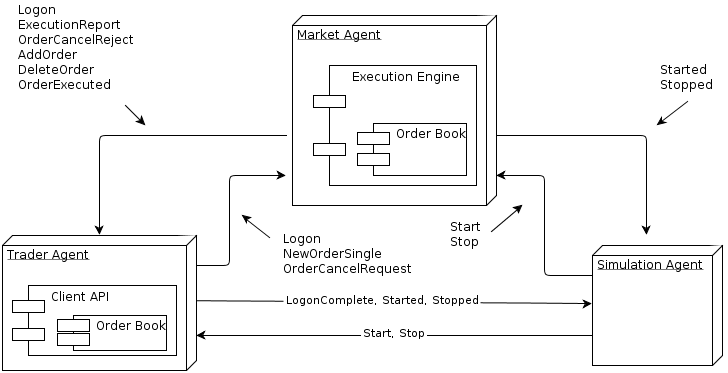
\includegraphics[scale=0.6]{Chapters/Analysis-and-Design/Design.png}}
\caption{Overall Design. The arrows refer to the names and flow of messages.}
\label{Figures/Analysis-and-Design/Design}
\end{figure}

\Cref{Figures/Analysis-and-Design/Design} shows the high-level design and messages exchanged between different agents. All messages explicitly carry the information about the agent that originates the message. 

The role of the Order Matching Engine is handled by the \texttt{Market Agent} that accepts all messages and passes the responsibility of processing the messages to the \texttt{Execution Engine}\footnote{\texttt{Execution Engine} is part of the \texttt{Market Agent}, therefore there are no actual messages exchanged, just method calls, see~\Cref{Chapters/Implementation/Market-Agent} for details}. Similarly, all market events (accepting a new order, executing orders, cancelling orders) are also disseminated by the \texttt{Market Agent} to \texttt{Trader Agents}. \texttt{Trader Agents} are simply the agents that simulate the participants in the market process. All orders submitted to the \texttt{Market Agent} need to carry a unique \texttt{ClOrdID} generated by the \texttt{Trader Agent} that sends the order. Whenever a market event is sent to the \texttt{Trader Agents} other than the original \texttt{Trader Agent} that submitted the order, unique \texttt{OrderID}s generated by the \texttt{Market Agent} are sent instead of the \texttt{ClOrdID}s (similarly all executions carry a unique \texttt{TradeID}, see~\Cref{Chapters/Background/Transparency}).

The simulation lifecycle is controlled by the \texttt{Simulation Agent} that is responsible for starting and stopping the simulation, in particular starting the \texttt{Market Agent} and \texttt{Trader Agents}, and letting the \texttt{Trader Agents} know the identity of the \texttt{Market Agent}. Additionally, the \texttt{Simulation Agent} can optionally send initial orders to the \texttt{Order Book}, before any \texttt{Trader Agent} starts sending orders. The initial orders are sent in order to stabilise the order book.

In order to simplify the low-level details of dealing with the \texttt{Market Agent} and the \texttt{Simulation Agent}, the \texttt{Trader Agents} use the \texttt{Client API} that provides a simple way to send and receive messages. In particular, the \texttt{Client API} handles the generation of unique \texttt{ClOrdID}s and provides several services like rebuilding the limit order book from the messages received from the \texttt{Market Agent}, so that \texttt{Trader Agents} can track the current prices and the overall situation on the market.